\section{Chart::LinesPoints}
\herv{Name:} Chart::LinesPoints\\ \\
\herv{File:} LinesPoints.pm\\ \\
\herv{Requires:}Chart::Base, GD, Carp, FileHandle\\ \\
\herv{Description:} \fett{LinesPoints} is a \fett{subclass} of Chart::Base.\\
The class LinesPoints creates a lines chart with points at the ends of the lines.\\
\\
\herv{Example:}
\begin{figure}[h]
	\begin{center}
		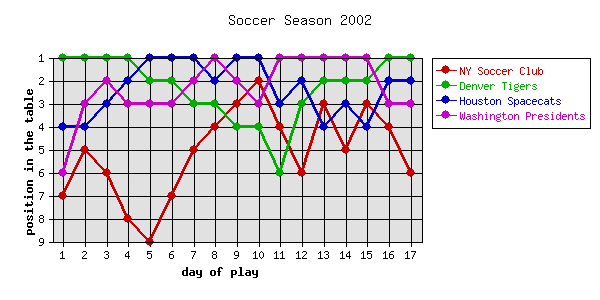
\includegraphics[scale=0.6]{d_linesp2.png}
	\end{center}
	\caption{Linespoints chart}
	\label{fig:d_linesp2}
\end{figure}
\begin{verbatim}
use Chart::LinesPoints;
use strict;

my (@data1, @data2, @data4, @data3, @labels, %hash, $g);

@labels = qw(1 2 3 4 5 6 7 8 9 10 11 12 13 14 15 16 17);
@data1 = qw (-7 -5 -6 -8 -9 -7 -5 -4 -3 -2 -4 -6 -3 -5 -3 -4 -6);
@data2 = qw (-1 -1 -1 -1 -2 -2 -3 -3 -4 -4 -6 -3 -2 -2 -2 -1 -1);
@data3 = qw (-4 -4 -3 -2 -1 -1 -1 -2 -1 -1 -3 -2 -4 -3 -4 -2 -2);
@data4 = qw (-6 -3 -2 -3 -3 -3 -2 -1 -2 -3 -1 -1 -1 -1 -1 -3 -3);

$g = Chart::LinesPoints->new(600,300);
$g->add_dataset(@labels);
$g->add_dataset(@data1);
$g->add_dataset(@data2);
$g->add_dataset(@data3);
$g->add_dataset(@data4);

%hash =(
          'integer_ticks_only' => 'true',
          'title' => 'Soccer Season 2002\n ',
          'legend_labels' => ['NY Soccer Club', 'Denver Tigers',
                              'Houston Spacecats', 'Washington Presidents'],
          'y_label' => 'position in the table',
          'x_label' => 'day of play',
          'grid_lines' => 'true',
          'f_y_tick' => \&formatter,
          );

$g->set ( %hash);
$g->png ("Grafiken/d_linesp2.png");

#just a trick, to let the y scale start at the biggest point:
#initiate with negative values, remove the minus sign!
sub formatter {
  my $label = shift;
  $label = substr($label, 1,2);
  return $label;
}

\end{verbatim}
\herv{Constructor:} An instance of a linespoints chart object can be created with the constructor new():\\
\fett{\$obj = Chart::LinesPoints->new();}\\
\fett{\$obj = Chart::LinesPoints->new(\kursiv{width}, \kursiv{height});}\\
\\
If \fett{new} has no arguments, the constructor returns an image with the size 300x400 pixels. If new has two arguments \kursiv{width} and \kursiv{height}, it returns an image with the desired size. \\ 
\\ 
\herv{Methods:}All universally valid methods, see page \pageref{methods}: Chart::Base. \\
\\
\herv{Attributes/Options:} All universally valid options, see page \pageref{options}. Also available these special options:
\begin{description}
\item['y\_axes'] Tells chart where to place the y-axis. Valid values are 'left', 'right' and 'both'. Defaults to 'left'.
\item['pt\_size']Sets the radius of the points in pixels. Default is 18.
\item['brush\_size']Sets the width of the lines in pixels. Default is 6.
\item['xy\_plot']Forces Chart to plot a x-y-graph, which means that the x-axis is also numeric if set to 'true'. Very useful for plots of mathematical functions. Defaults to 'false'.
\item['sort']Sorts the data of a x-y-graph ascending if set to 'true'. Should be set if the added data isn't sorted. Defaults to 'false'.  
\end{description}
